% taylor-couette.tex

\section{Taylor Couette Flow}
\label{taylor-couette}
%
Some test cases for taylor couette flow are simulated, this could be used to verify 
the rotational speed pf Moving wall boundary condition. A journal paper titled "Monta Carlo
and Navier-Stokes Simulations of Compressible Taylor-Couette Flow" is found and used as test
cases, and three different pressure were simulated, namely, low pressure ($10Pa$), intermediate
pressure ($100Pa$) and high pressure ($1000Pa$). Experimental data used for the simulation is
shown in Table~\ref{ex_data}

\begin{table}
  \caption{Experimental data for simulation}
  \label{ex_data}
  \begin{center}
    \begin{tabular}{cccc}
     \hline
     \hline
     Test cases & intermediate pressure & high pressure & low pressure \\
     Inner radius, $m$ & 0.2125 & 0.2125 & 0.2125 \\
     Gap width, $m$ & 0.0031 & 0.0031 & 0.0031 \\
     Rotor Speed, $rpm$ & 27600 & 27600 & 27600 \\
     Rotor Temperature, $K$ & 348 & 351 & 344 \\
     Stator Temperature, $K$ & 350 & 366 & 344 \\
     Taylor Number & 17 & 181 & 3.6 \\
     \hline
     \hline
    \end{tabular}
  \end{center}
\end{table}

\medskip
To simulate this test case, only a small portion of geometry is stidied, then periodic boundary
condition with different orientations is applied. For the low and intermediate pressure cases,
since the taylor number is quite low, there is no vortices generated, then the grid is low resolution
at $z$ direction, while for high pressure case, the vortices might be generated along the axial gap,
and results in high resolutie at $z$ direction.

\begin{figure}[htbp]
\begin{center}
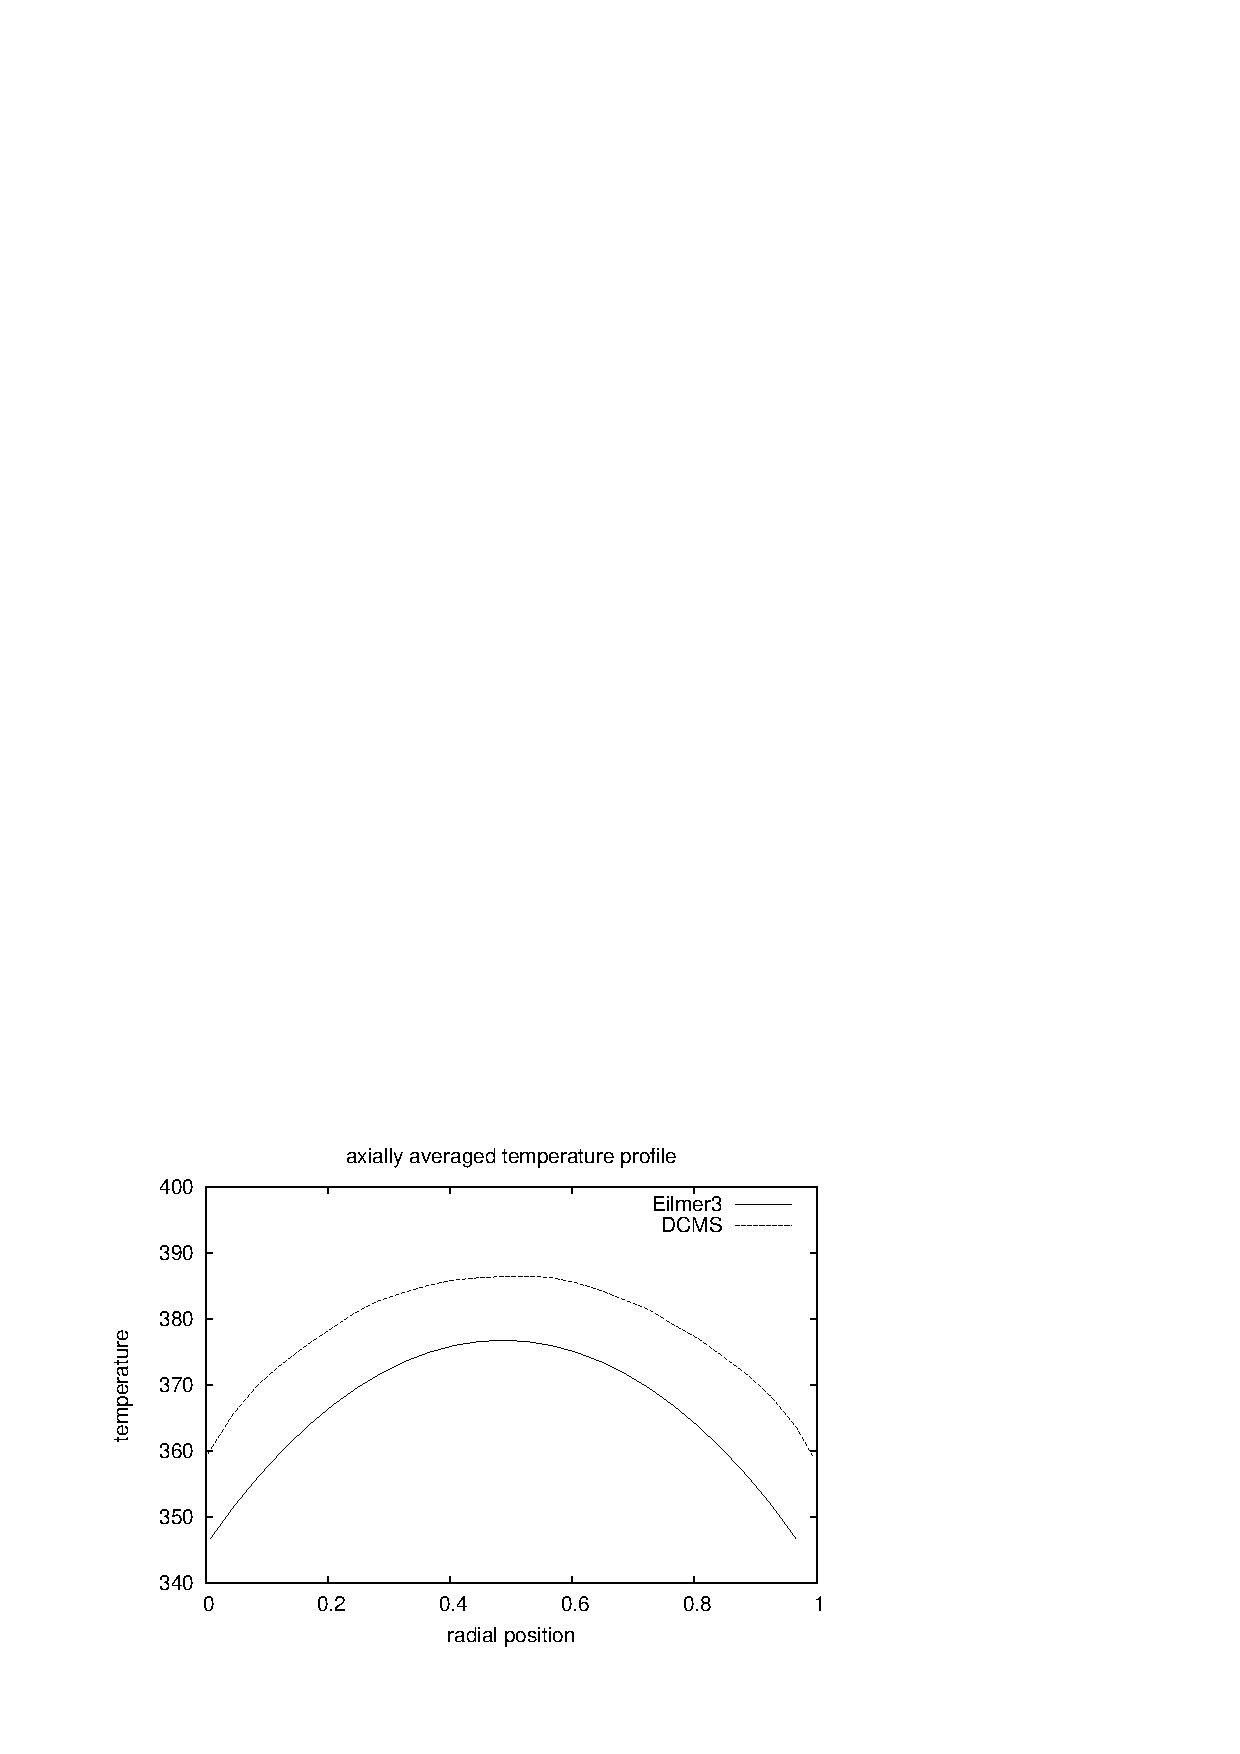
\includegraphics[width=0.45\textwidth,viewport=41 46 411 298,clip=true]{../3D/taylor-couette/temperature-low.pdf}
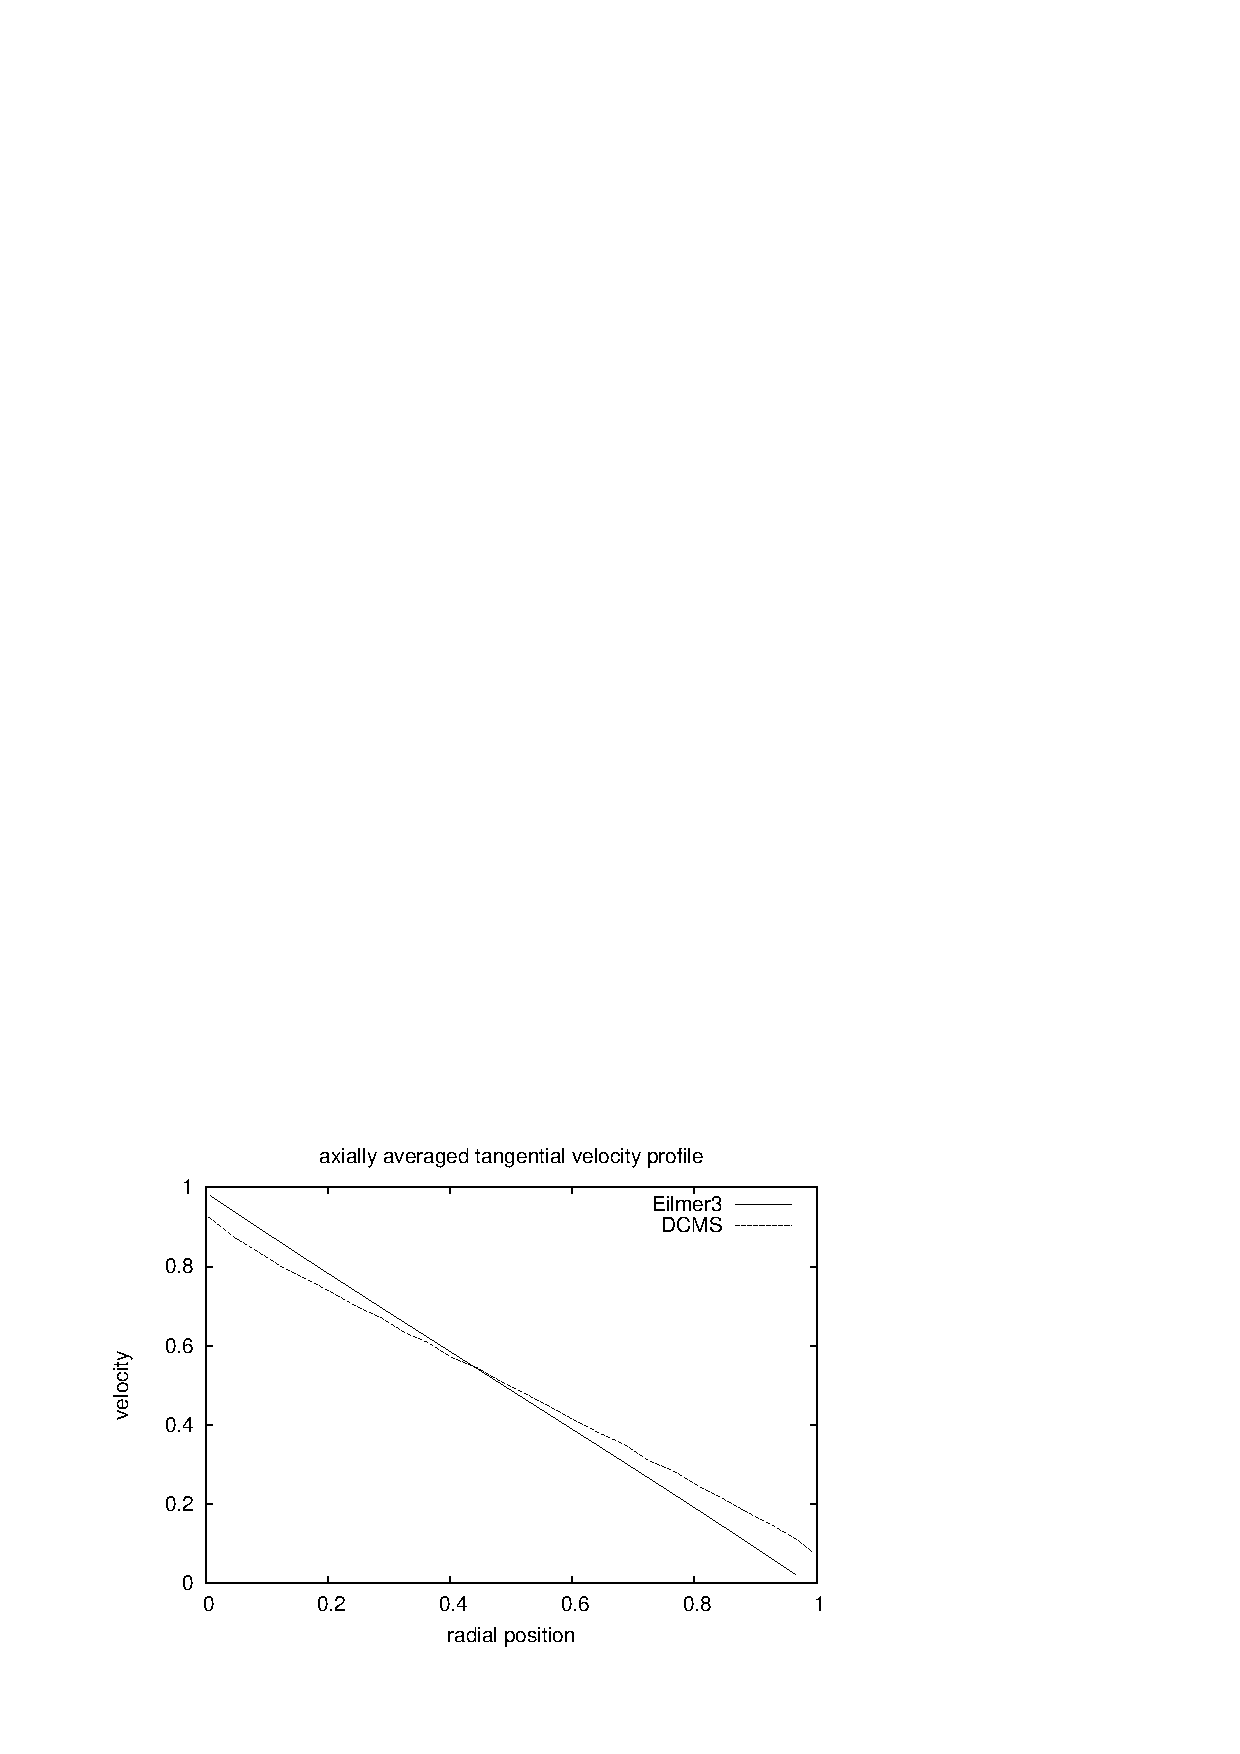
\includegraphics[width=0.45\textwidth,viewport=41 50 407 303,clip=true]{../3D/taylor-couette/velocity-low.pdf}
\end{center}
\caption{Comparison of temperature and velocity profiles along radial direction at low pressure condition.}
\label{tcl-tv-fig}
\end{figure}

\medskip
For the low pressure case, the velocity profile is roughly linear accross the narrow gap, and the temperature
profile has a parabolic shape with maximum temperature near the center of the gap. Figure~\ref{tcl-tv-fig}
indicate the comparison results of velocity and temperature with different methods.
The apparent differecne is that the slip wall boundary condition is considered in DSMC method. However, with pressure
increases, the wall can be regarded as no-slip condition.

\begin{figure}[htbp]
\begin{center}
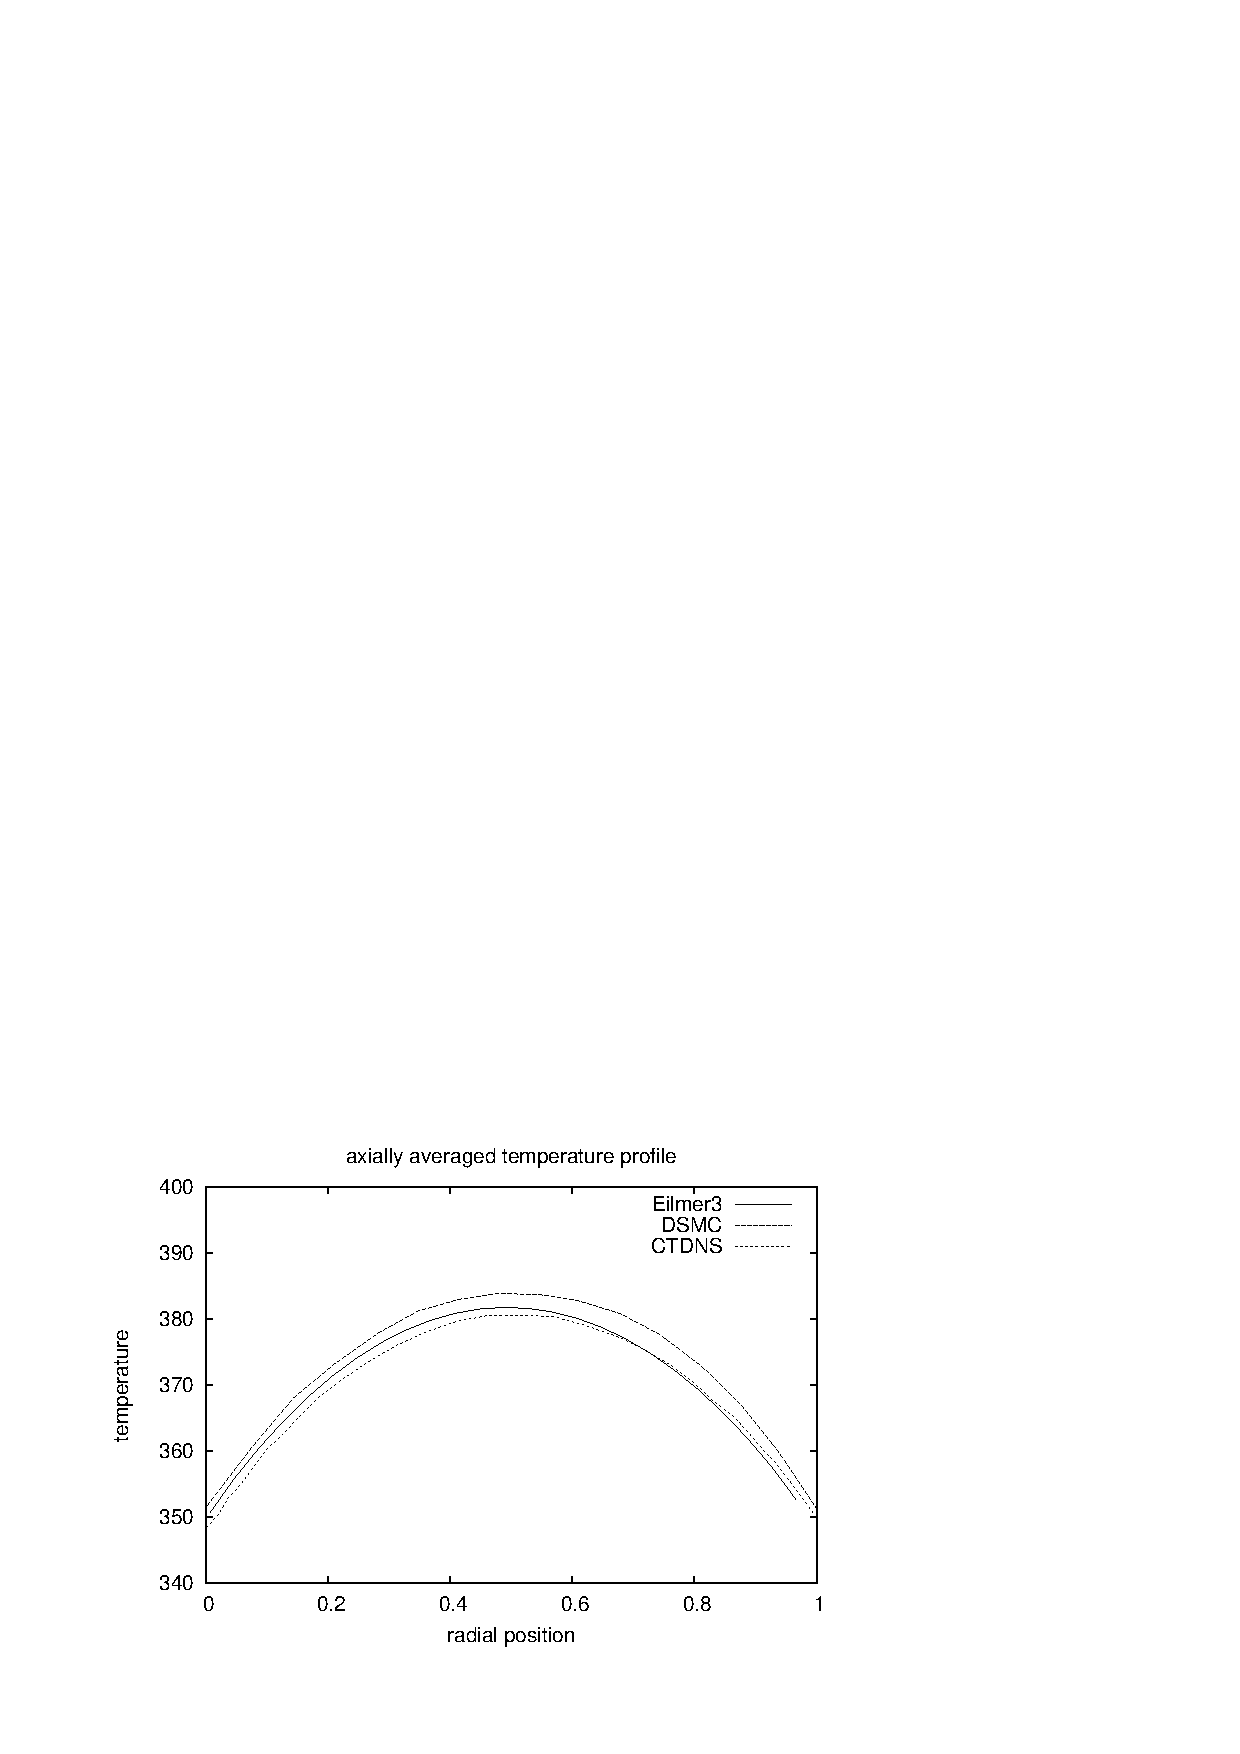
\includegraphics[width=0.45\textwidth,viewport=41 46 411 298,clip=true]{../3D/taylor-couette/temperature-intermediate.pdf}
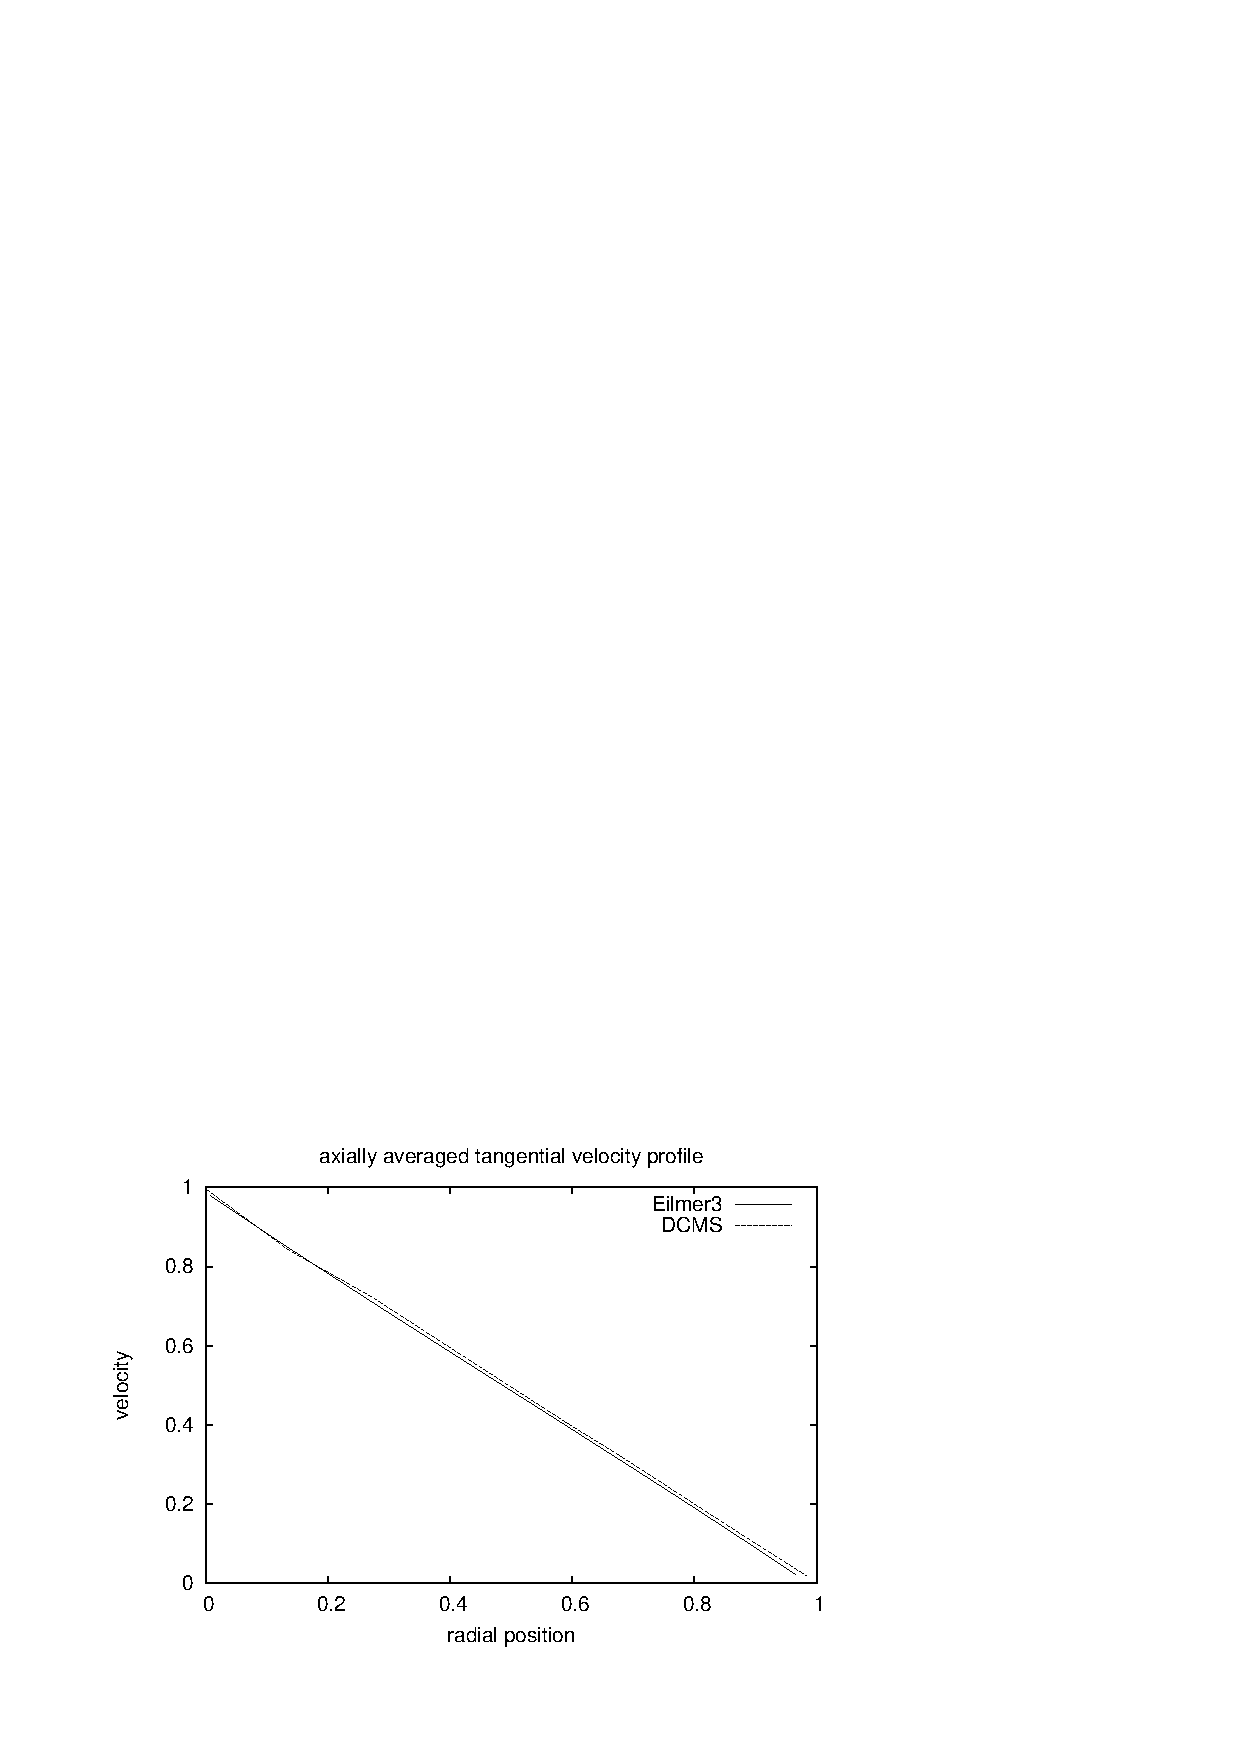
\includegraphics[width=0.45\textwidth,viewport=41 50 407 303,clip=true]{../3D/taylor-couette/velocity-intermediate.pdf}
\end{center}
\caption{Comparison of temperature and velocity profiles along radial direction at intermediate pressure condition.}
\label{tci-tv-fig}
\end{figure}

\medskip
For the intermediate pressure case, there is the same situation with low pressure, which are shown in
Figure~\ref{tci-tv-fig}. The profile for the tangential velocity is nearly linear
and the temperature profile is nearly parabolic with a maximum slightly closer to the hotter wall as seen in
Figure~\ref{tci-tv-fig}. The agreement between numercial results is good.

\begin{figure}[htbp]
\begin{center}
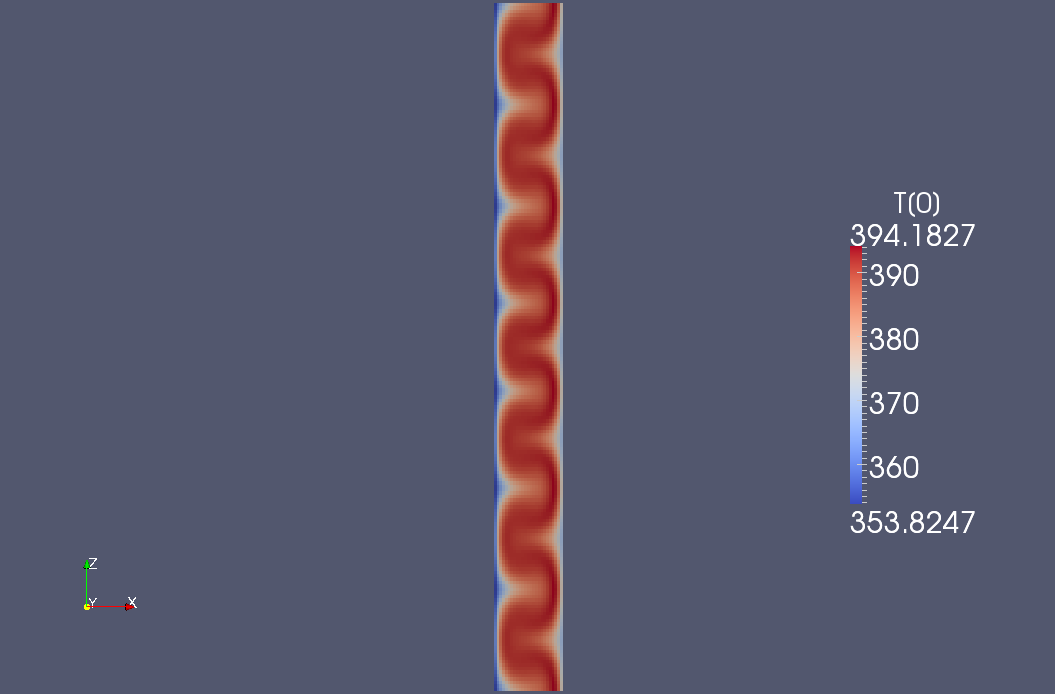
\includegraphics[width=0.45\textwidth]{../3D/taylor-couette/temperature.png}
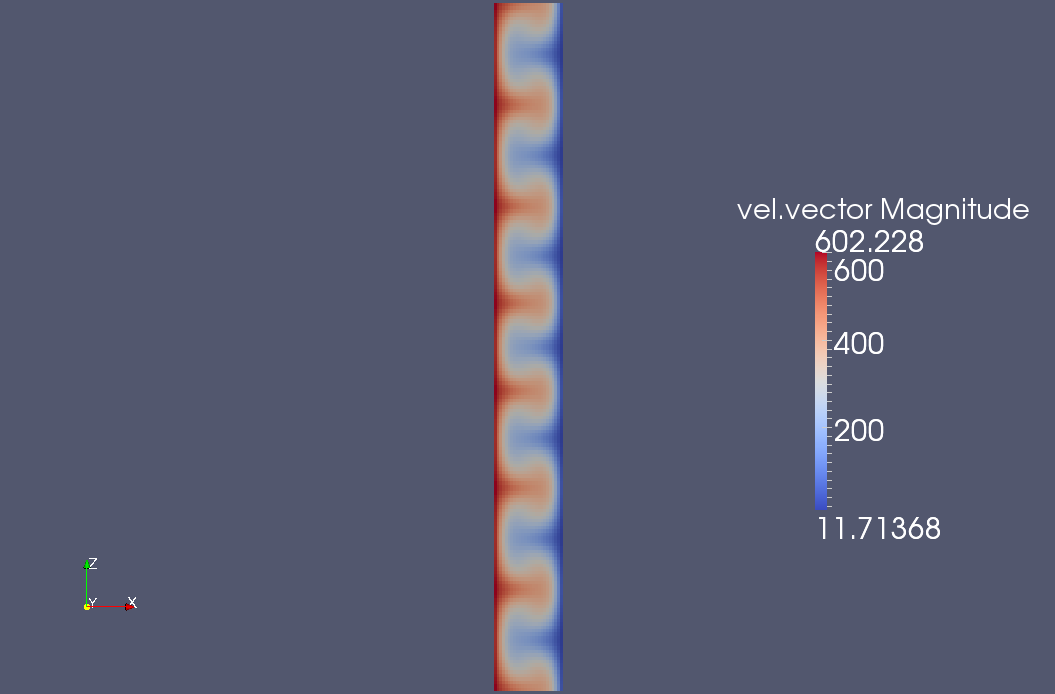
\includegraphics[width=0.45\textwidth]{../3D/taylor-couette/velocity.png}
\end{center}
\caption{Temperature contour at high pressure condition.}
\label{tv-fig}
\end{figure}

\medskip
For the high pressure case, since taylor number has reached to a certain level, there is vortices generated.
Figure~\ref{tv-fig} show velocity and temperature contour at high pressure
condition, and clearly vortices are generated along the axial gap.

\begin{figure}[htbp]
\begin{center}
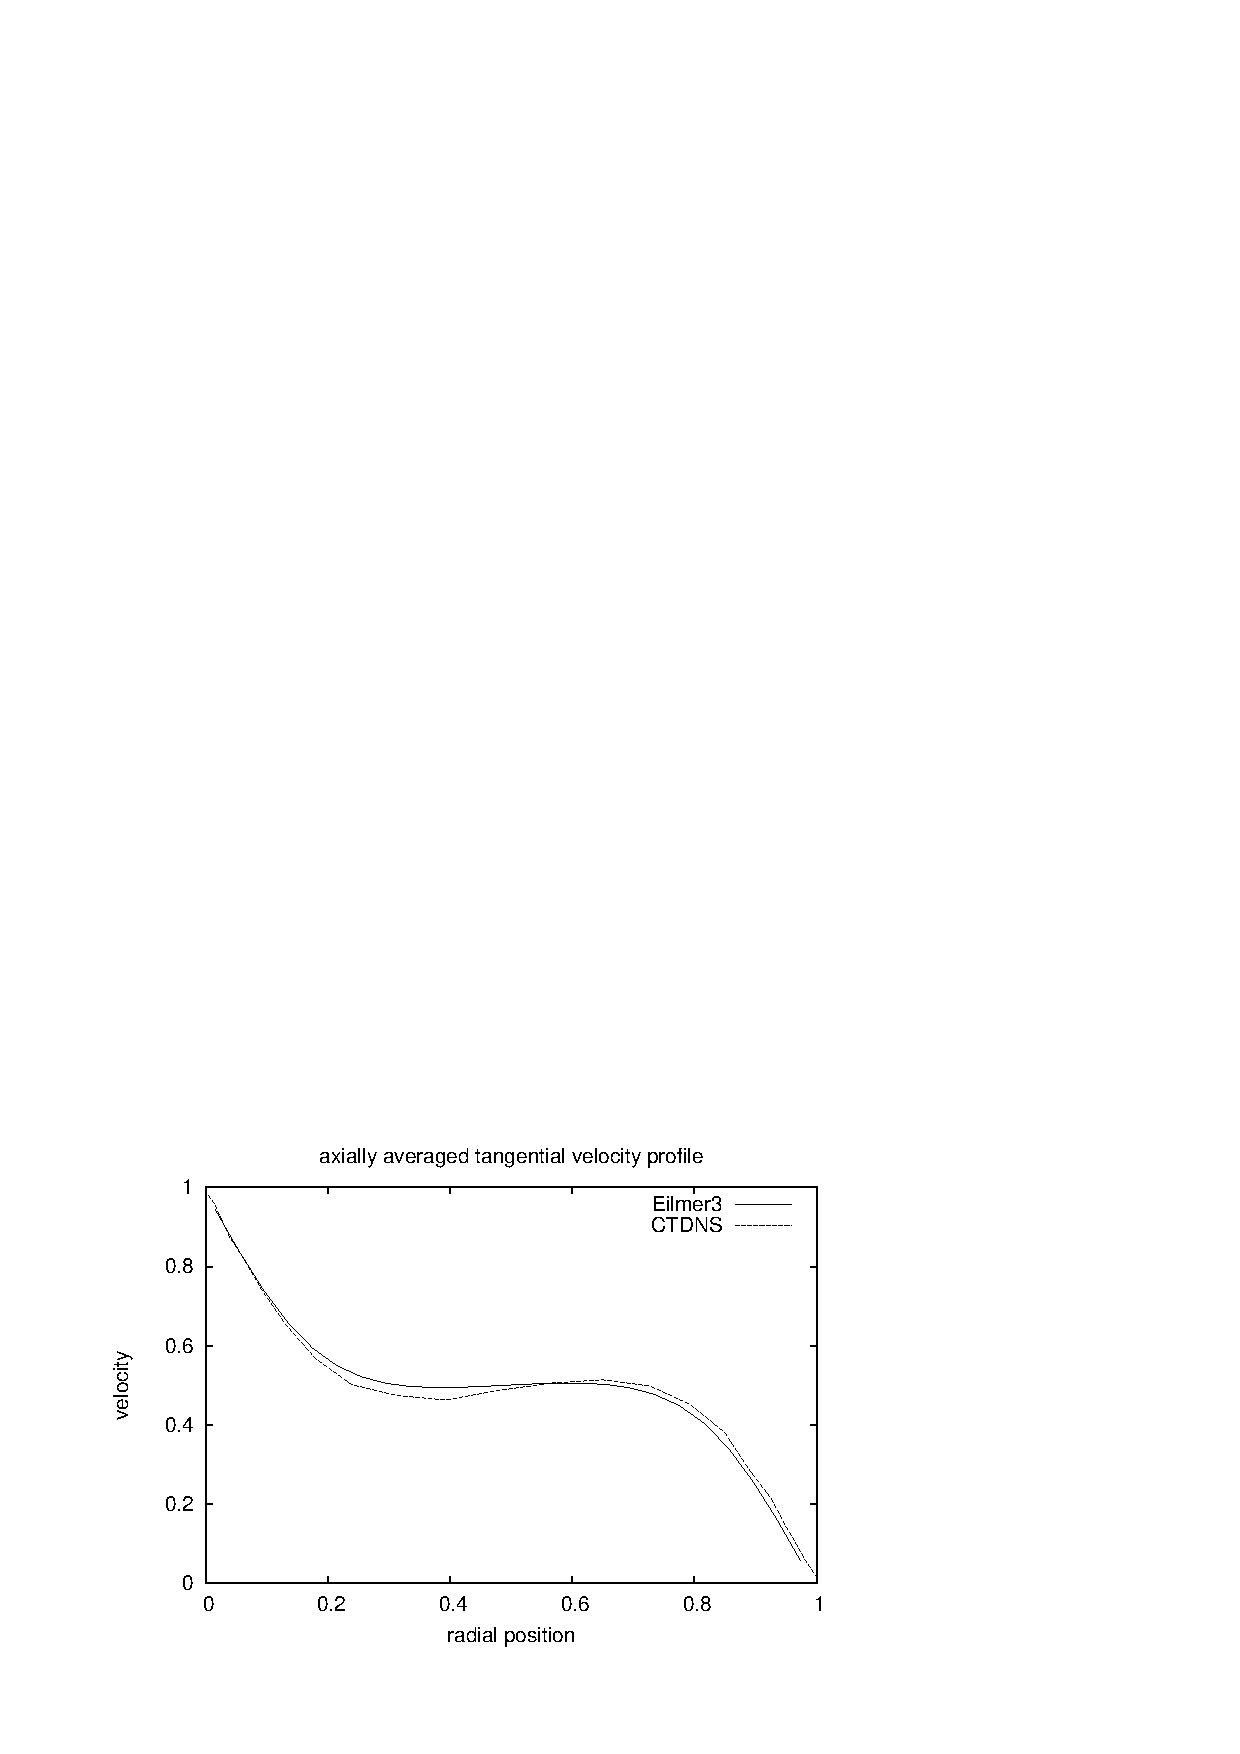
\includegraphics[width=0.8\textwidth,viewport=41 50 407 303,clip=true]{../3D/taylor-couette/velocity-high.pdf}
\end{center}
\caption{Comparison of velocity profiles along radial direction at high pressure condition.}
\label{tch-velocity-fig}
\end{figure}

\medskip
The velocity profile has evolved into an "S-shape" curve (see in Figure~\ref{tch-velocity-fig}) in the axially averaged 
flow due to the presence of vorticesin the gap. The "S-shape" of the velocity profile characterizes a flow with a higher 
gradient at the walls due to mixing induced by the vortices and a nearly flat region where the axially averaged velocities 
are nearly constant in the middle of the gap.

\begin{figure}[htbp]
\begin{center}
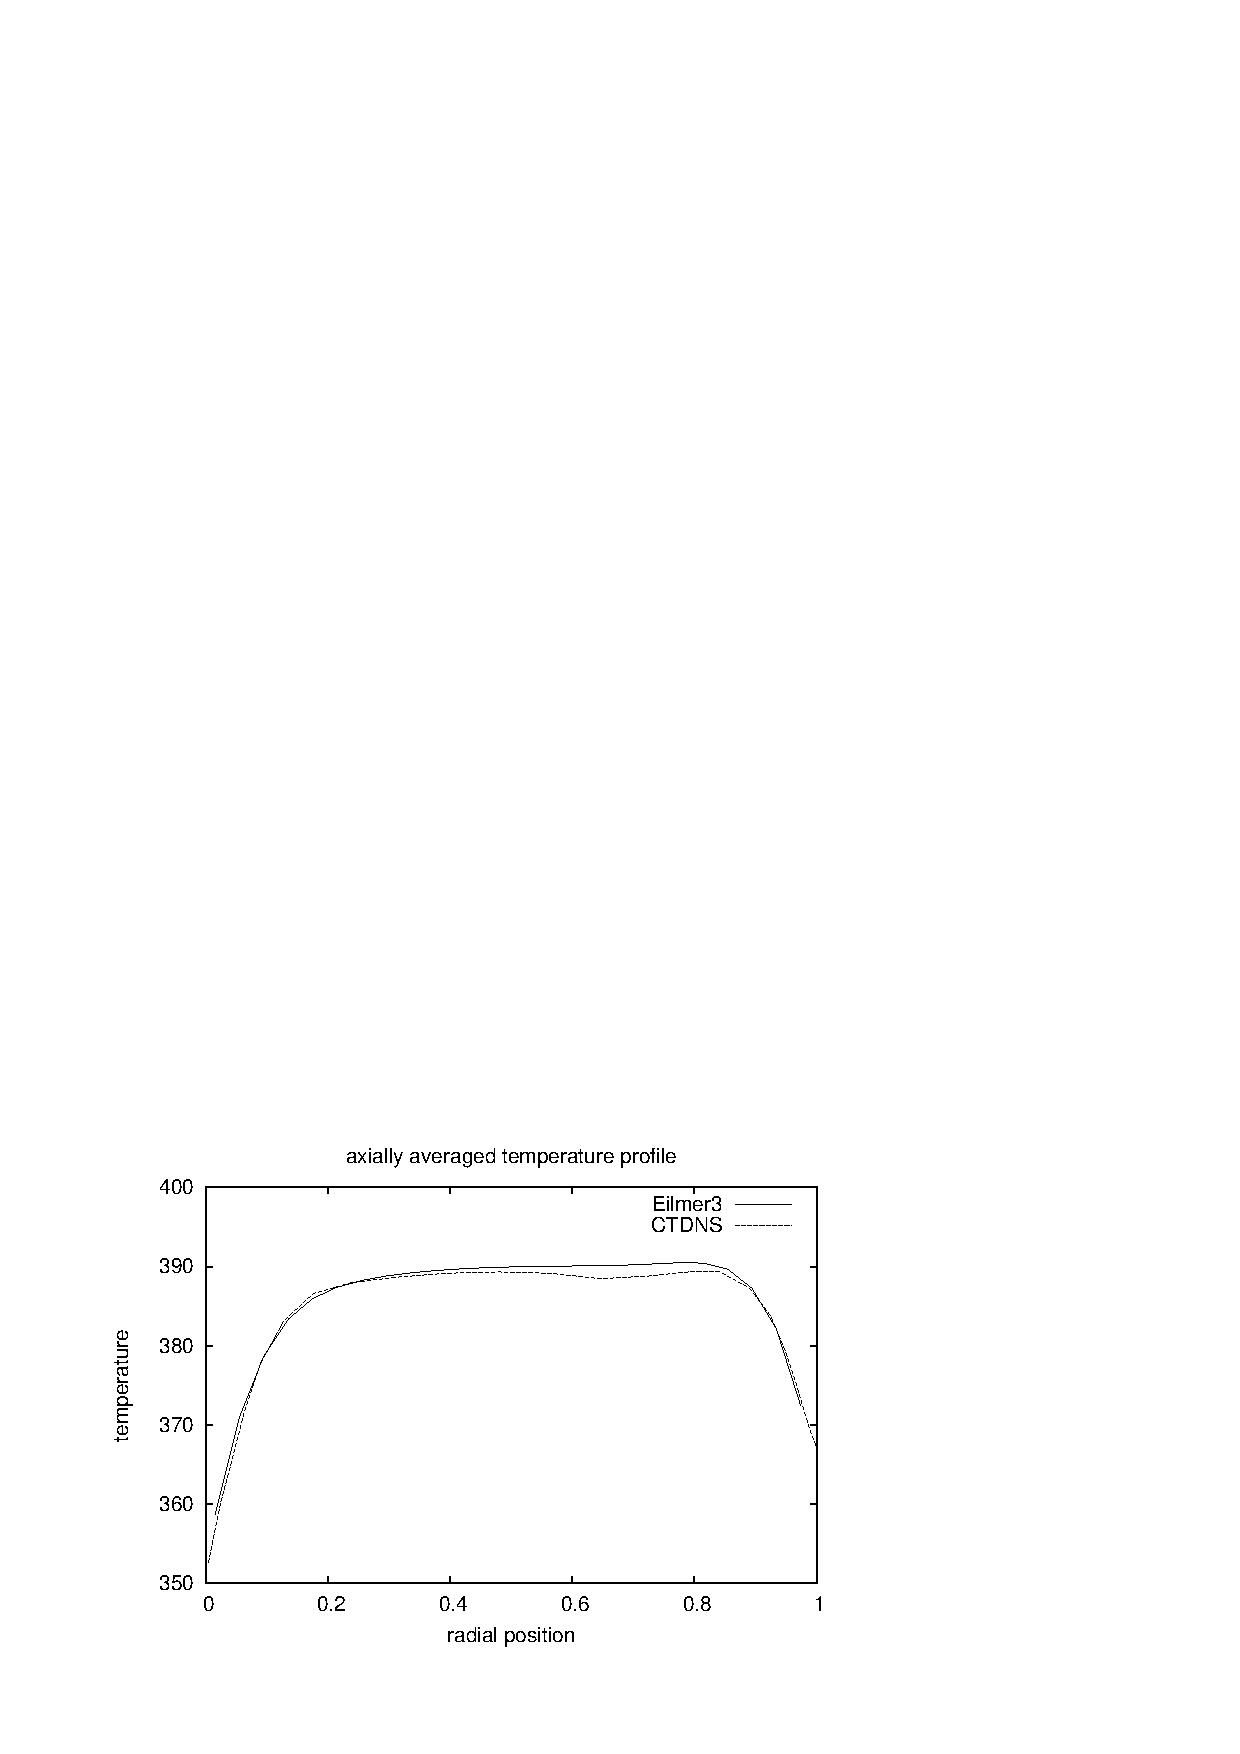
\includegraphics[width=0.8\textwidth,viewport=41 46 411 298,clip=true]{../3D/taylor-couette/temperature-high.pdf}
\end{center}
\caption{Comparison of temperature profiles along radial direction at high pressure condition.}
\label{tch-temperature-fig}
\end{figure}

\medskip
The axially averaged temperature profile (seen in Figure~\ref{tch-temperature-fig}) exhibits two peaks, the highest of which 
is closer to the hottest wall. Theshape in the center of the gap is much flatter than in the laminar flows. This averaged shape 
also exhibits steeper graidentsat the walls, which will induce a high heat flux. All these changes are due to the presence of 
vortices taht cause macroscopic radial mixing of the flow.

\newpage
\subsection{Input script (.py)}
\topbar
\lstinputlisting[language={}]{../3D/taylor-couette/tc_flow_nitrogen.py}
\bottombar


\subsection{Shell scripts}
\label{tc-sh-files}
\topbar
\lstinputlisting[language={}]{../3D/taylor-couette/prep.sh}
\bottombar

\noindent
\topbar
\lstinputlisting[language={}]{../3D/taylor-couette/tc_flow_nitrogen.sh}
\bottombar

\noindent
\topbar
\lstinputlisting[language={}]{../3D/taylor-couette/post.sh}
\bottombar

\subsection{Notes}
\begin{itemize}
\item Python script for calculating axially averaged temperature and velocity profile.
      \lstinputlisting[language={}]{../3D/taylor-couette/a_vt.py}
\end{itemize}
